\documentclass[11pt, a4paper]{article}

\usepackage{amsmath}
\usepackage{amsfonts} %Matheschriften
\usepackage{amssymb} %Mathesymbole
%\usepackage{mathptmx} % Einstellung für Schriften und Sonderzeichen in mathematischen Umgebungen
                        % ändert SChriftfont
\usepackage{wasysym} % Stellt diverse Sonderzeichen bereit
\usepackage{siunitx}
\usepackage{float}
\usepackage{microtype}
\usepackage{graphicx}
\usepackage{hyperref}
\usepackage{xcolor}
\usepackage[section]{placeins}
% allows for temporary adjustment of side margins
\usepackage{changepage}
%\usepackage{rotating}


\usepackage[ngerman]{babel}
\addto\captionsngerman{%
 \renewcommand{\abstractname}{Einleitung}}

\title{Versuch 6: Zustandsgleichung reller Gase}
\author{Jascha Fricker, Benedict Brouwer}

\begin{document}
    \maketitle

    

    \begin{abstract}
        Dieser Versuch beschäftigt sich mit dem Verhalten von Gasen bei verschiedenen Drücken und Temperaturen.
        Dabei wird nicht nur bei niedrigem Druck das gasförmige Verhalten untersucht, sondern auch bei hohem Druck
        der Übergang zur flüssigen Phase.
    \end{abstract}

    \tableofcontents

    \newpage

    \section{Theorie}
    Wenn bei niedrigem Druck die Wechselwirkung zwischen den Gasmolekülen vernachlässigt werden kann,
    kann das Verhalten eines Gases sehr gut mit der idealen Gasgleichung
    \begin{align}
        p V &= n R T \nonumber \nonumber\\
        n &= \frac{p V}{R T} \label{eq:ideal}
    \end{align}
    (Siehe \cite[(1)]{ZUS}) beschrieben werden. So kann bei gegebenem Druck $p$, Temperatur $T$, Volumen $V$,
    Gaskonstanten $R$ und die molare Stoffmenge $n$ bestimmt werden. \\

    Wenn hingegen die Wechselwirkung zwischen der Teilchen $a$ mit dichtester Kugelpackung $b$
    berücksichtigt werden soll, gilt die Van der Waals Gleichung \cite[(4)]{ZUS}:
    \begin{align}
        \left(p+\left(\frac{n}{V}\right)^2 \cdot a\right) \cdot \left(V-n \cdot b \right) = n \cdot R \cdot T
    \end{align}
    Diese Gleichung beschreibt auch den Phasenübergang von gasförmig zu flüssig bei niedrigen Temperaturen.
    Wenn man den Druck p gegen das Volumen bei konstanter Temperatur aufträgt, entsteht ein sogenannter Isotherm.
    Dieser hat bei nierdigen Temperaturen zwei Extrema und einen Wendepunkt. 
    Eine wichtiger Parameter eines Gases ist die kritische Temperatur $T_{krit}$, bei der Isothermen dieser Temperatur
    fallen Wendepunkt und Extrema zu einem Sattelpunkt zusammen.
    Mithilfe der kritischen Temperatur und dem kritischen Druck können die Parameter
    \begin{align}
        b &= \frac{V_{krit}}{3n} \label{eq:b}\\
        a &= 27 \cdot \left(\frac{V_{krit}}{3n}\right)^2 \cdot p_{krit} \label{eq:a}
    \end{align} 
    berechnet werden.
    Für $T < T_{krit}$ gibt es bei der Isothermen ein Bereich,
    wo die Messwerte nicht der Kurve folgen, sondern ein konstantes Wert entsteht. Dieser wird als Dampfdruck $p_{d}$
    bezeichnet. Hier liegen sowohl Flüssigkeit als auch Gas vor. Die Höhe dieser Geraden kann auch rechnerisch durch die Maxwell-Konstruktion bestimmt werden.
    Der Zusammenhang zwischen Dampfudruck und Temperatur kann mit der Clausius-Clapeyron-Gleichung \cite[(9)]{ZUS} beschrieben werden.
    \begin{align}
        \frac{d p_d}{d T} = \frac{L}{T \cdot\left(V_g - V_{fl}\right)} \label{eq:delta}
    \end{align}
    mit Verdampfungsenthalpie $L$, Gasvolumen $V_g$ und Flüssigkeitsvolumen $V_{fl}$.

    \section{Experimentelles Vorgehen}
    In dem Messaufbau konnte das Volumen der Küvette, in dem das Gas Schwefelhexaflourid eingeschlossen wurde, verändert und gemessen werden.
    Die Temperatur wurde durch ein Wasserbad auf einer konstanten Temperatur gehalten und durch ein Thermometer gemessen. 
    Der Druck in der Küvette wurde mithilfe eines Manometers gemessen.

    \section{Ergebnisse}
    \subsection{Stoffmenge}
    \begin{figure}
        \centering
        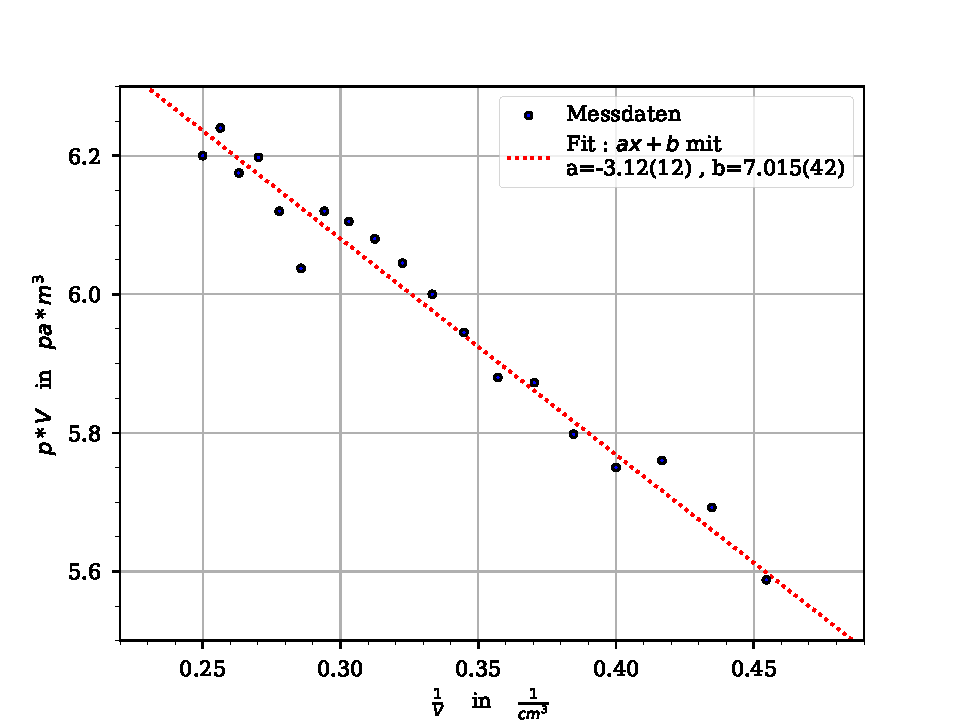
\includegraphics[width=\textwidth]{./Plots/3Plot_n.pdf}

        \caption{Bestimmung der molaren Stoffmenge $n$}
        \label{fig:n}
    \end{figure}
    
    Mithilfe der genauen Messreihe bei $50 \si{\celsius}$ wurde durch einen Fit der
    Funktion \ref{eq:ideal} im Graph \ref{fig:n} die molare Stoffmenge $n = 0,002613(16) \si{\mole}$ bestimmt.
    Diese molare Masse wurde für alle Messreihen benutzt.

    \subsection{Isotherme}
    
    \begin{sidewaysfigure}
        \centering
        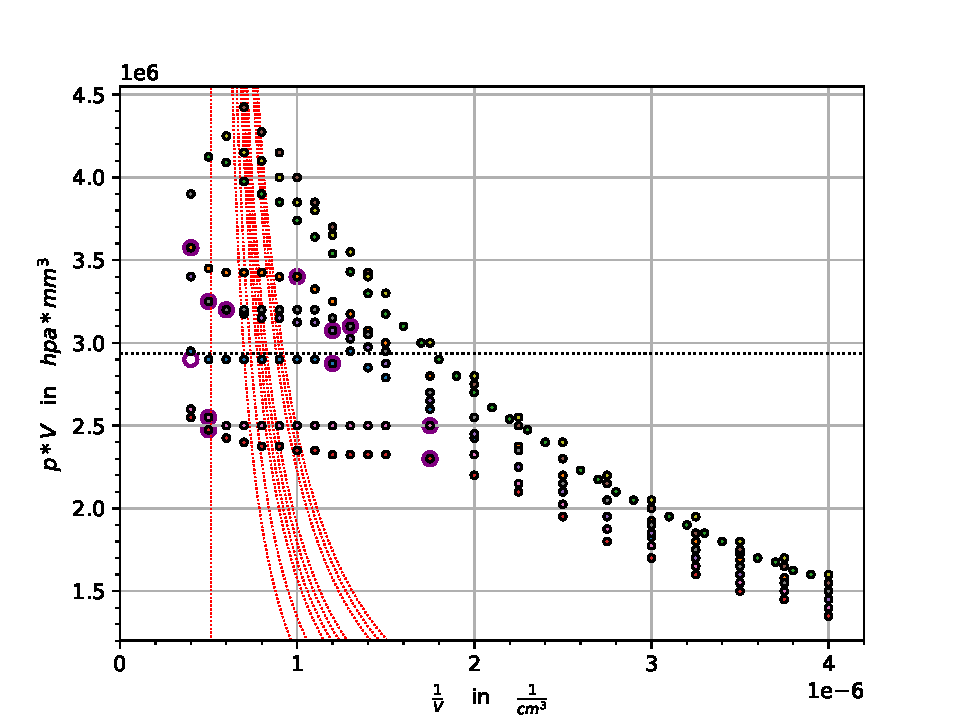
\includegraphics[width=\textwidth]{./Plots/4Plot_of_Hell.pdf}

        \caption{Isotherme bei verschiedenen Temperaturen}
        \label{fig:isotherme}
    \end{sidewaysfigure}
    Die Isotherme sind im Graphen \ref{fig:isotherme} dargestellt, wobei der Druck gegen das Volumen aufgetragen wurde.
    Die Punkte an denen nur noch Gas bzw. Flüssigkeit vorhanden ist, wurden mit einem Kreis markiert. Als
    Unsicherheit wurde die Schrittweite des Thermometers ($\Delta T = 0,1 \si{\celsius} \Rightarrow u_t = 0,028 \si{\celsius}$)
    der Volumenmessung ($\Delta V = 0,05 \si{\milli\liter} \Rightarrow u_v = 0,011 \si{\milli\liter}$) und der Druckmessung
    ($\Delta p = 0,5 \si{\hecto\pascal} \Rightarrow u_p = 0,11 \si{\hecto\pascal}$) verwendet (Berechnung der Unsicherheiten 	mittels Dreiecks- bzw. Rechtecksverteilung)
    Die Bereiche in denen das Schwefelhexaflourid nur flüssig, gasförmig oder gemischt vorliegt, wurden mit verschiedenen
    Farben im Graphen \ref{fig:isotherme} hervorgehoben.

    \subsection{Kritischer Punkt}

    Aus dem Graphen \ref{fig:isotherme} kann anhand der Ausgleichsfunktion durch die Randbereiche der Phasen
    die kritische Temperatur $T_{krit}$ , das kritische Volumen $V_{krit}$ und der kritischen Druck $p_{krit}$ bestimmt werden.
    
    \begin{table}
        \centering
        \begin{tabular}{c}
            Literatur \\ \hline
            $T_{krit} SF_6 = 45,55 \si{\degree \celsius}$ \cite{SH6} \\
            $p_{krit} SF_6 = 37,53 \si{\bar}$ \cite{SH6} \\
            $\rho_{krit} SF_6 = 735 \si{\kilogram \per \meter \cubed}$ \cite{SH6} \\
            \\
            Messwerte \\ \hline
            $p_{krit} = 3,51 \si{\mega\pascal}$ \\
            $V_{krit} = 0,693 \si{\centi\metre\cubed}$ \\
            $\rho_{krit} = \frac{n \cdot M}{V} = 551 \si{\kilogram \per \meter \cubed}$ \\
            $a_{mol} = 0,7406(91) \frac{Pa m^6}{mol^2}$ \\
            $a_{Teilchen} = 1.229(15)*10^{-24} \frac{Pa m^6}{mol^2}$ \\
            $b_{mol} = 8.840(55)\si{\cubic\metre\per\mol}$\\
            $b_{Teilchen} = 1.4679(90)*10^{-28} \si{\cubic\metre\per\mol}$
        \end{tabular}
        \caption{kritischer Punkt}
        \label{tab:krit}
    \end{table}
    Anhand des Parameter b kann überlegt werden, dass ? sozusagen das Volumen der "Hülle" eines einzelnen Teilchens ist.
    \subsection{Dampfdruck}
    \begin{figure}
        \centering
        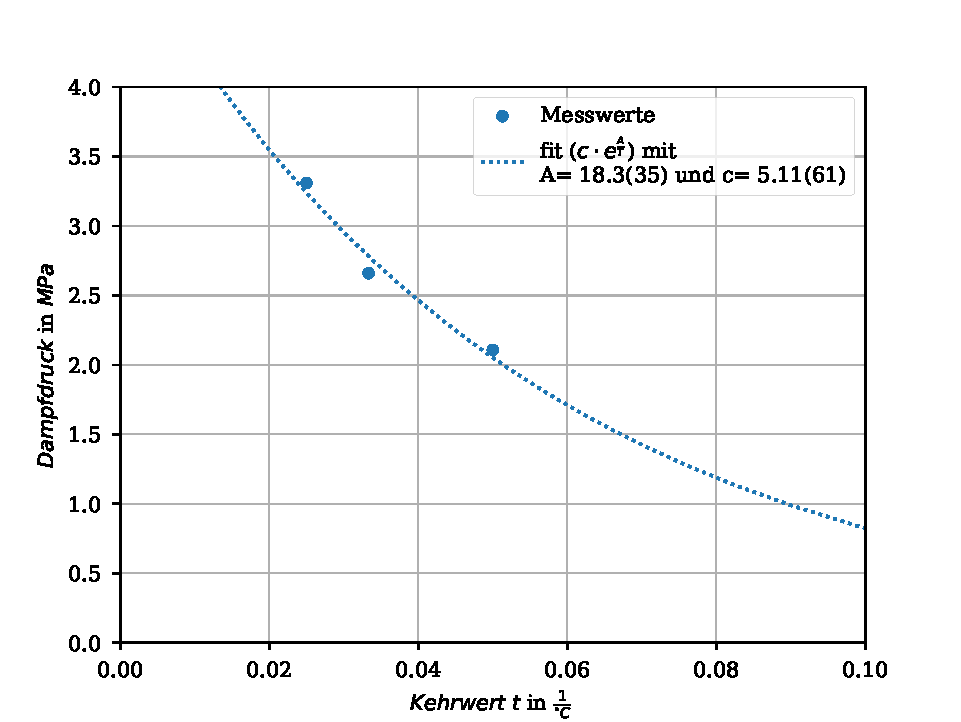
\includegraphics[width=\textwidth]{./Plots/dampf.pdf}

        \caption{Dampfdruck}
        \label{fig:dampf}
    \end{figure}

    Der Dampfdruck bei verschiedenen Temperaturen konnte durch die Höhe der geraden Teilbereiche
    der Isothermen in \ref{fig:isotherme} bestimmt werden.
    

    Durch fitten des Verhältnisses zwischen $p$ und $T$ durch die Exponenitalfunktion
    \begin{align}
        p_d = c \cdot e^{-\frac{A}{T}},
    \end{align}
    welche im Graph \ref{fig:dampf} dargestellt ist,
    kann die Ableitung der Exponenitalfunktion berechnet werden. So kann mit \ref{eq:delta}
    die Verdampfungsenthalpie $L$ bestimmt werden. Diese Werte sind in Tabelle \ref{tab:dampfmess}
    aufgelistet. In \ref{fig:verd} wird die Verdampfungsenthalpie $L$ verglichen mit Temperatur $T$ dargestellt.
    \begin{table}
        \begin{adjustwidth}{-.5in}{-.5in}
        \centering
        \begin{tabular}{c c c c c}
            Temperatur & Dampfdruck & $V_g$ & $V_fl$ & Verdampfungsenthalpie $L$ \\ \hline
            $25.0 \si{\celsius}$ & $23.5 \si{\hecto\pascal}$ & $670 \si{\milli\litre\per\mole} $ & $ 190  \si{\milli\litre\per\mole} $ & $ 1038 \si{\joule\per\mole} $ \\
            $30.0 \si{\celsius}$ & $25.0 \si{\hecto\pascal}$ & $670 \si{\milli\litre\per\mole} $ & $ 190  \si{\milli\litre\per\mole} $ & $ 1017 \si{\joule\per\mole} $ \\
            $35.2 \si{\celsius}$ & $29.0 \si{\hecto\pascal}$ & $460 \si{\milli\litre\per\mole} $ & $ 150  \si{\milli\litre\per\mole} $ & $ 625 \si{\joule\per\mole} $ \\
            $37.5 \si{\celsius}$ & $31.4 \si{\hecto\pascal}$ & $460 \si{\milli\litre\per\mole} $ & $ 190  \si{\milli\litre\per\mole} $ & $ 535 \si{\joule\per\mole} $ \\
            $40.0 \si{\celsius}$ & $31.8 \si{\hecto\pascal}$ & $500 \si{\milli\litre\per\mole} $ & $ 230  \si{\milli\litre\per\mole} $ & $ 523 \si{\joule\per\mole} $ \\
            $42.4 \si{\celsius}$ & $34.2 \si{\hecto\pascal}$ & $380 \si{\milli\litre\per\mole} $ & $ 150  \si{\milli\litre\per\mole} $ & $ 437 \si{\joule\per\mole} $
        \end{tabular}
        \caption{Ergebnisse Dampfdruck und Verdampfungsenthalpie}\label{tab:dampfmess}
        \end{adjustwidth}
    \end{table}
    \begin{figure}
        \centering
        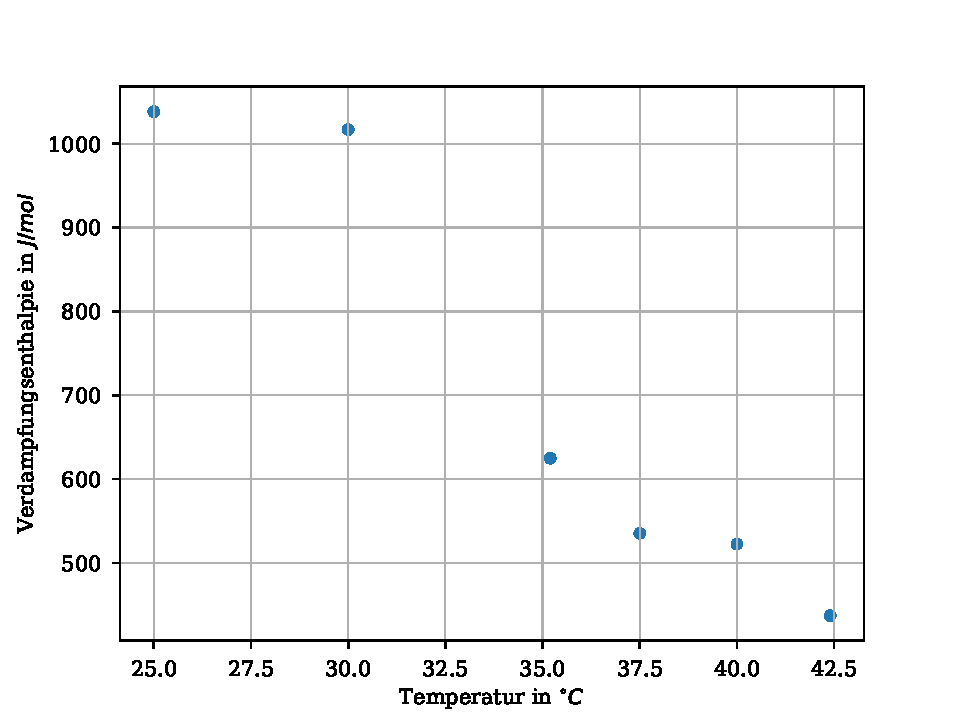
\includegraphics[width=\textwidth]{./Plots/verd.pdf}

        \caption{Verdampfungsenthalpie}
        \label{fig:verd}
    \end{figure}
    \section{Diskussion}
    \subsection{Isotherme}
    Leider konnten die Isothermen nicht durch die Theoriefunktion gefittet werden, wir haben uns auch dagegen entschieden die 
    Messpunkte zu verbinden, da so ein falscher Eindruck entstehen könnte. Die Daten zu den verschiedenen Phasenübergängen waren 
    nicht genau, wie in \ref{fig:isotherme} zu sehen. Auch kann es sein, dass manchmal nicht lang genug vor der 
    Messung gewartet wurde, sodass sich die Temperatur nicht ausgeglichen hatte und falsche Messwerte abgelesen wurden.
    Diese Fehler schlagen sich natürlich auch auf die nachfolgenden Berechnungen der charakteristischen Werte aus.

    \subsection{Kritischer Punkt}
    In Tabelle \ref{tab:krit} werden die kritischen Werte für $SF_6$ aus der Literatur aufgelistet.
    \begin{table}
        \centering
        \begin{tabular}{c}
            $T_{krit} SF_6 = 45,55 \si{\celsius}$ \cite{SH6} \\
            $p_{krit} SF_6 = 37,53 \si{\bar}$ \cite{SH6} \\
            $\rho_{krit} SF_6 = 735 \si{\kilogram \per \meter \cubed}$ \cite{SH6} \\
            \\
            \begin{tabular}{c c}
                Temperatur in $\si{\degree\celsius}$ & Dampfdruck in $\si{\bar}$ \\ \hline
                20 \si{\celsius} & 2,108 \si{\mega\pascal} \\
                30 \si{\celsius} & 2,66 \si{\mega\pascal} \\
                40 \si{\celsius} & 3,31 \si{\mega\pascal} \\
            \end{tabular}
        \end{tabular}
        \caption{Literaturwerte}
        \label{tab:literaturwerte}
    \end{table}
    Beachtet man die ungenaue Bestimmungsmethoden, sind die Messwerte vergleichsweise nah an an den Literatuwerten.

    \subsection{Dampfdruck}
    Wie im Graph \ref{fig:dampf} zu sehen liegen die Literaturwerte des Dampfdrucks relativ weit von den Messwerten.
    Bei der Verdampfungsenthalpie hingegen gibt es sehr große Sprunge im Graphen, und obwohl die Ausgleichsfunktion
    uns nicht bekannt ist, haben die berechneten Werte wahrscheinlich sehr große Fehler.

    \subsection{Fehler durch zu kleine Zeit zwischen den Messungen}

    Wenn das Volumen des Gases verkleinert bzw. vergrößert, dann erhitzt sich das Gas bzw. es kühlt ab.
    Da die Messungen jedoch bei konstanter Temperatur durchgeführt werden müssen, muss vor 
    der nächsten Messung das Gas erst wieder vom Wasserbad abgekühlt bzw. erhitzt werden. Sonst verfälscht
    eine zu große bzw. kleine Temperatur die Messwerte.
    


    \bibliographystyle{plain}
    \bibliography{literature}

\end{document}